\documentclass[10pt,conference,compsocconf]{IEEEtran}

\usepackage{hyperref}
\usepackage{graphicx}	% For figure environment
\usepackage{mathptmx}
\usepackage{helvet}
\usepackage{courier}
\usepackage{graphicx}
\usepackage{imakeidx} \makeindex[options = -s svind]
\usepackage{multicol}
\usepackage[bottom]{footmisc}
\usepackage{natbib}
\bibliographystyle{humannat}
\usepackage{amssymb}
\usepackage{amsmath}
\usepackage{float}
%\restylefloat{table}
%\usepackage{floatrow}
%\floatsetup[table]{capposition=top}
%\usepackage{lscape}
\usepackage{breqn}
%\usepackage{listings}
\usepackage{color}
%\usepackage[utf8]{inputenc}
%\usepackage{array}
%\definecolor{mygreen}{RGB}{28,172,0}
%\definecolor{mylilas}{RGB}{170,55,241}

\newcommand{\plim}{\text{plim}}
\newcommand{\tr}{\text{tr}}
\newcommand{\diag}{\text{diag}}
\newcommand{\rank}{\text{rank}}
\newcommand{\Exp}{\text{E}}
\newcommand{\vect}{\text{vec}}
\newcommand{\vech}{\text{vech}}
\newcommand{\Var}{\text{Var}}
\newcommand{\lnf}{\text{ln f}}
\newtheorem{assumption}{Assumption}
\usepackage{amsmath}
\usepackage{breqn}
\newcommand{\R}{\mathbb{R}}

\begin{document}
\title{Project 1}

\author{
  Monika Avila Marquez \\
  \textit{EPFL}
}

\maketitle

\begin{abstract}
  
\end{abstract}	\textbf{We develop a classification model that allows to determine whether the decay observed corresponds to a Higgs Boson particle or to another one. We propose a boosted linear regression model and a logistic one. For the former, we estimate the vector of weights using least squares method which aims to minimize the MSE. For the latter, we use the maximum likelihood method modified by adding a random vector. This modifications avoids convergence to local minima. Additionally, we only update the weights if we have an improvement of the loss function. }

\section{Introduction}

The aim of this project is to develop a classification model for the decay processes observed. Such that we are able to predict if they correspond either to a Higgs Boson particle or to another one. For this purpose, we propose to use a  boosted linear regression model and a logistic one. For the former, we estimate the vector of weights using least squares method which aims to minimize the MSE . Then, we create a new variable which captures the mistakes done in the prediction in the first estimation. Using this new variable we aim run a second round of linear regression. The aim is to reduce the prediction error. For the latter, we use the maximum likelihood method. For the maximization of the likelihood we use Gradient Descent that we modify by adding a standard gaussian d-dimensional vector which allows to avoid to be converge to local minima. Additionally, we only update the weights if we have an improvement of the loss function.
We obtain , as we could have predicted, that the best method is the logistic regression. We obtain nearly 70\% of predictions that were done correctly. 
However, we consider that we could have improved the methods by using a radial basis with a gaussian kernel. Nevertheless, due to time pressure and complexity of the method we leave this improvement for later.
\section{The Model}
\label{S1}
In order to estimate the likelihood that an event signature is the result of a High boson process, we model the data using a boolean variable called $y_i, \forall i \in  \{1, 2, ..., 2500\}  $ as:

 $$
y_{i}=
\begin{cases}
1, & \text{if} \quad prediction_i=b\\
0, & \text{otherwise}
\end{cases}
, 
$$
Since the expectation of a boleaan variable is equal to the probability that the variable is equal to 1, we can model the probability that the event is the result of a High Bosson process with a linear model:
$$p_w(y_i=1|\textbf{x}_i)=E(y_i|\textbf{x}_i)=\textbf{x}'_i w$$
Where $\textbf{x}_i $ is a vector of D attributes considered in the regression and $w \in \R^D $ are the weights.
However, as it is well known the biggest pitfall of this model is the fact that the estimated probability is out of the boundaries of the closed interval $ ( 0,1 ) $. 
In order to address the problem mentioned, we use the logistic regression. This model lies within the framework of a Generalized Linear Model.  In this case, the probability of having a HB process is modeled as following:
$$p_w(y_i=1|\textbf{x}_i)=\frac{\exp(\textbf{x}'_i w)}{1+exp(\textbf{x}'_i w)}$$
For purposes of simplicity and because it is well known, we don't present the expression of the likelihood of the model.
\section{Methods}
In the previous section, we have presented the models that we used. Now, we will describe the methods employed for the estimation of the vector of weights $w$. Since we have two different models, the estimation technique will be different. 
For the linear regression model, we use Ordinary Least Squares method aiming to minimize the MSE. For this, we used the normal equations and the closed from solution for the weights. 
For the logistic regression model, we aim to maximize the likelihood. For this we used Gradient Descent. We modified the gradient descent method by adding a d-dimensional gaussian random vector such that we avoid convergence to local minima. 
$$w^{m+1}=w^{m}-\lambda  \nabla \l(w^m) +v^{m+1}$$
with $v^{m+1} \sim d-Gaussian(0,I)$. Where $I$ is a DxD identity matrix and 0 a vector of zeros in $\R^D$.
Moreover, we add the condition that we ill update the weight in each iteration only if the loss function is lower than in the previous step. While it is true that adding this condition increases the computational burden, the benefit is that we improve our prediction results since we reach better convergence.

\section{The Data}
\label{S1}
In this section, we will discuss the data used to test and compare the models that mentioned above. Our training dataset consists of 250.000 instances for 30 features and 1 output variable. The latter indicates if the decay corresponds to a Higgs boson particle collision event or from other event. The dataset is generated from simulation which mimics the actual particle collision events in which Higgs bosons (with fixed mass 125GeV) were produced and 3 other background processes. 

The set of features consist of both raw data which were measured by actual sensors and derived quantities computed from raw features. We can see the statistical description of first 5 features in table \ref{Table2}. We can conclude that the standard deviation is extremely high. This is why we also standardized the features. Moreover, in figure \ref{fig1} we study the separability of signal from background on a sample of 2 features. Here, it is clear that there is an overlapping thus the selection of features is important. 

%{\tiny \begin{table}[htb]
%	\addtolength\tabcolsep{2pt}
%	\caption{Descriptive Statistics}
%	\label{Table 1}
%	\addtolength\tabcolsep{2pt}
%	\begin{tabular}{llrrrrr}
%		\hline\noalign{\smallskip}
%	Variable 	& Min. & Max. & 1st Quartile  \\
%		\noalign{\smallskip}\hline\noalign{\smallskip}
%		 mass_MMC   				& -999.00 	& 1192.03	& 78.10 	 \\
%	mass_transverse_met_lep	& 0.000 	& 690.08 		& 19.24 	  \\                        
%	mass_vis						& 6.33  		& 1349.35 	& 59.39	 	\\   
%	pt_h								& 0.00 		& 2834.99 	& 14.069	\\
%	deltaeta_jet_jet				& -999.00 	& 8.50	& -999.00 	\\
%		\noalign{\smallskip}\hline\noalign{\smallskip}\\
%	\end{tabular}
%\end{table}
\begin{table}[htb]	\label{Table2}
	\addtolength\tabcolsep{2pt}
	\caption{Descriptive Statistics}
	\addtolength\tabcolsep{2pt}
	\begin{tabular}{llrrrrr}
		\hline\noalign{\smallskip}
		Variable 	& 3d Quartile & Mean & St. Dev. \\
		\noalign{\smallskip}\hline\noalign{\smallskip}
mass_MMC   				&  130.61	 & -49.02 &406.35 \\
mass_transverse_met_lep	 	& 73.59 	& 49.24 &35.34 \\                        
mass_vis						 	&92.26 & 81.18 & 40.83\\                        
pt_h							& 79.17		& 57.89 & 63.66\\
deltaeta_jet_jet			 	&0.49		& -708.42 & 454.48 \\                         
		\noalign{\smallskip}\hline\noalign{\smallskip}\\
	\end{tabular}
\end{table}
%\begin{tiny}
%		\begin{figure}[b]
%			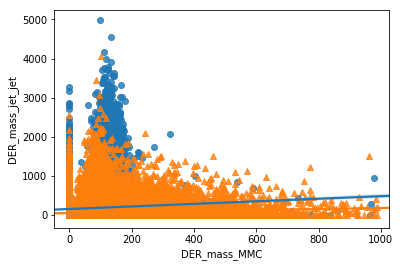
\includegraphics[scale=0.5]{separ.png}   
%			\caption{Separability of the training set }
%			\label{fig1}    
%		\end{figure}
%\end{tiny}

Even though we have considerably large variation of features almost 70\% of all events lack at least one feature. In order to solve this problem, we used an imputation method using the mean values of the respective feature. The goal is to minimize the effects of missing data. 

And finally, we have applied 2 discriminative transformations. First we used polynomial terms up to second order. Secondly, we obtained the sinus and cosine of the feature. As a result, we obtained 90 features including the original ones. From this new set, we have selected the best combination of features with a forward selection method. This method consisted on an iterative process, in each iteration we chosed the best regressors based on the ones that reduced MSE the most. %(See figure \ref{fig2})
\begin{tiny}
	\begin{figure}[t]
		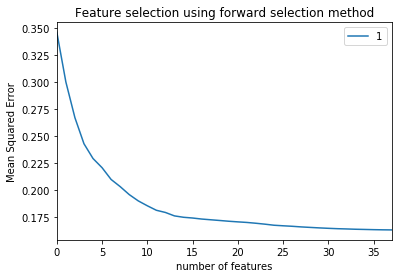
\includegraphics[scale=0.5]{Mse.png}   
		\caption{Result of forward selection method }
		\label{fig2}    
	\end{figure}
\end{tiny}


\section{Results}
\label{S1}
To test and compare each 6 regression functions proposed we need to have general testing method. First, we divided our dataset 80\% for training and 20\% on testing. And then, we used actual prediction error rate on testing dataset, instead of MSE or likelihood to measure model's performance. In figure \ref{fig3}, we can see the relationship between error rate and number of training iteration (note that least regression and ridge_regression doesn't require iteration). 

\begin{tiny}
	\begin{figure}[b]
		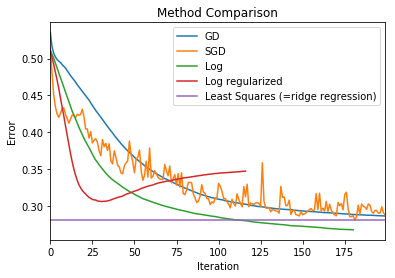
\includegraphics[scale=0.5]{MethodComp.png}   
		\caption{Separability of the training set }
		\label{fig3}    
	\end{figure}
\end{tiny}

From the figure 3 we can see that logistic regression converges into much lower error rate (0.22) while other linear regressions converge into 0.26. However, least squares method considerably high performance using much lower computational expense than that of logistics.
\section{Discussion}
\label{S1}
  In our approach we have used solid feature selection method which filtered most effective features from large pool. By removing outliers the best threshold value to quantize the result of regression stabilized at 0.5 in any linear regression. In addition, we compared our result with gradient boosting using least squares method. Apparently, gradient boosting converged into same result of single least squares method.
  Since we've proved using sigmoid function results better performance, there is possibility of improving our model much further by using different exponential functions.
\section{Summary}
\label{S1}
In this project we propose a boosted linear regression in which we aim to correct the mistakes of the predictions done in a first round by creating a new variable which is used as the dependent regressor in a second round. The method performs better than the simple linear regression. However, logistic regression outperforms this method. This is expected since this model allows to model the probability within the closed interval (0,1). 
We encountered difficulties regarding the selection of the best futures and the best basis. We used a polynomial basis and aimed to do sinusoidal basis. However, we consider that using a radial basis or a spline basis would have improved the results. The spline basis has as advantage that the features are orthogonal which allows to reduce distortions in the estimation, small singular values in the design matrix. Thus, we would aim to introduce this improvements in further research. 


\end{document}